% @Author: AnthonyKenny98
% @Date:   2020-03-01 18:51:24
% @Last Modified by:   AnthonyKenny98
% @Last Modified time: 2020-04-10 06:28:06
\subsection{RISC-V}

    \glsdesc{RISC-V} (pronounced ``risk-five'') was developed at the University of California, Berkeley. It is established on the principles of RISC as an open-source and extendable \gls{ISA} for research and education. It was designed with application specific processors in mind, as they developed a highly flexible and extendable base \gls{ISA} around which research and acceleration efforts could be based.

    The motiviation behind designing RISC-V was largely due to the disadvantages of commercially popular \glspl{ISA}.\cite{Isa2012} (Following list adapted from RISC-V ISA Manual).
    \begin{itemize}
    \item \textbf{Commercial ISAs are proprietary.} Owners of commercial ISAs carefully guard their intellectual property and will not share implementations. 
    \item \textbf{Commercial ISAs come and go.} Many once-popular commercial ISAs have since fallen out of fashion or are not even in production any more. Lingering intellectual property issues interefere with the ability of third-parties to continue supporting the ISA. While an open source \gls{ISA} may also lose popularity, interested parties can continue to use and support the ISA without interference.
    \item \textbf{Popular commercial ISAs were not designed for extendibility.} There exist almost no ISAs that support extendibility for general purpose computing systems, allowing for no application specific optimizations at the instruction set level.
    \end{itemize}

    RISC-V is designed cleverly in a modular way, with a set of base instruction sets and a set of standard extensions. As a result, processors can be designed to only implement the instruction groups it requires, saving time, space and power on instructions that won't be used. In addition, another goal of RISC-V is to provide a basis for more specialized instruction-set extensions or more customized accelerators. This is described in the most recent \textit{RISC-V Instruction Set Manual} \cite{Waterman2019}. This is a powerful feature, as it does not break any software compatability, but allows for designers to easily follow the steps outlined in Figure \ref{fig:extendingRISCV}. From a \gls{hardware acceleration} point of view, this is particularly useful as it allows the designer to directly invoke whatever functional unit or accelerator they implement from assembly code.
    
    % @Author: AnthonyKenny98
% @Date:   2020-03-01 10:28:34
% @Last Modified by:   AnthonyKenny98
% @Last Modified time: 2020-03-01 10:32:45
\begin{figure}[H]
\begin{center}
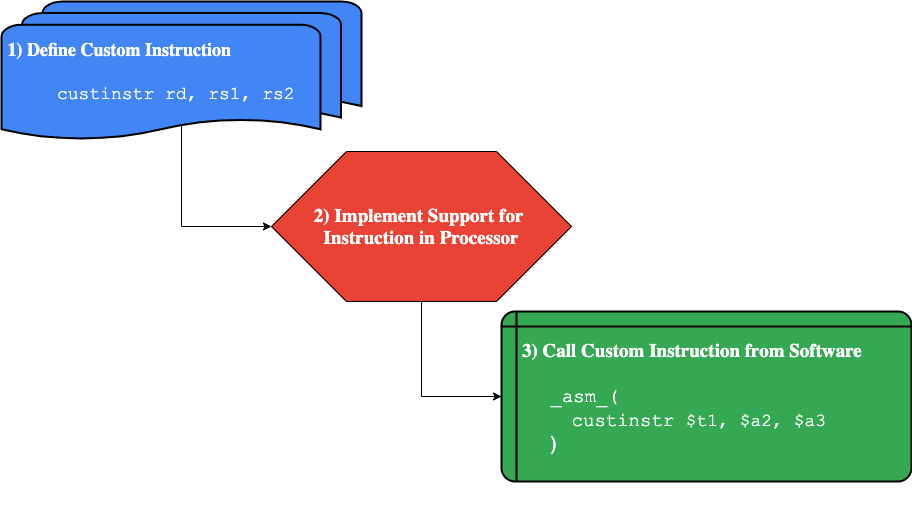
\includegraphics[width=0.9\linewidth]{chapters/chapter1/img/extendingRISCV.png}
\caption{Typical Process of Adding Non-Standard Extension to RISC-V ISA}
\label{fig:extendingRISCV}
\end{center}
\end{figure}

    The overall design of RISC-V can be broken down into 3 characteristics that address the aforementioned limitations of commercial \glspl{ISA}: Open-source, extendibility, and modularity.

    \subsubsection{Open-Source}
        Open-source refers to software of which the owner has granted permission for anybody to study, alter, and distribute the software for any purpose. Often, this means projects are developed in a collaborative public manner. What this means for and ISA is that the RISC-V implementations are often publically available and improved on by developers for their own purposes. Building a high-performance processor from scratch is an arduous, expensive project. Open-source implementations allow for developers to build off existing implementations without all the legwork of implementing a processor from scratch.

    \subsubsection{Extendability}
        RISC-V is designed to be extendable. This means that developers can add their own instructions to the Instruction Set and implement those new instructions in a processor. This processor should still be able to run all other RISC-V compiled programs, along with a set of programs for which it is specially optimized. This level of backwards compatibility means that an extended ISA is not just a new ISA. 

    \subsubsection{Modularity}
        Finally, RISC-V was designed to be relatively easy to implement. It is broken down into small ``base'' \glspl{ISA} which can then have any number of standard and custom extensions added to them. These base ISAs are not designed in such a way to overarchitect for a certain type of microarchitecure. This modularity and flexibility is part of what makes it such an attractive proposition for specialized computer architecture. Figure \ref{fig:modules} demonstrates this modularity.

        % @Author: AnthonyKenny98
% @Date:   2020-04-09 12:52:23
% @Last Modified by:   AnthonyKenny98
% @Last Modified time: 2020-04-09 20:19:52
\begin{figure}[H]
\begin{centering}
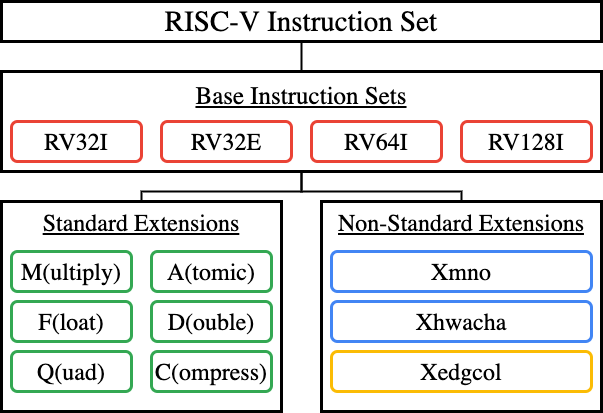
\includegraphics[width=0.8\linewidth]{chapters/chapter4/img/modules.png}
\mycaption{RISC-V ISA Modularity}{. It is clear that the RISC-V ISA is in fact a family of ISAs. Each is based on one of the ``base'' ISAs, which are each the smallest possible ISA to run just about any program. For more instructions and thus, better performance, any number of Standard or Non-Standard Extensions can be implemented on top of a base ISA.}
\label{fig:modules}
\end{centering}
\end{figure}

\subsection{RV32I}
    The RV32I (Short for RISC-V 32-Bit Integer) base \gls{ISA} is a small \gls{ISA} of only 40 unique instructions, but sufficient to support modern operating systems. It has 32 registers, \texttt{x0-x32}, each 32-bits wide. \texttt{x0} is a hard-wired 0, and there is also another register dedicated for the program count. 


    The following is an excerpt from the RISC-V Specification, outlining the RV32I base integer instruction set \cite{Waterman2019}
    \begin{quote}{}
        \small{RV32I was designed to be sufficient to form a compiler target and to support modern operating system environments. The ISA was also designed to reduce the hardware required in a minimal implementation. RV32I contains 40 unique instructions, though a simple implementation might \dots [reduce] base instruction count to 38 total. RV32I can emulate almost any other ISA extension \dots \\
        Subsets of the base integer ISA might be useful for pedagogical purposes, but the base has been defined such that there should be little incentive to subset a real hardware implementation \dots}
    \end{quote}

    % \subsubsection*{Registers}
    %     RV32I defines 32 unprivileged registers, each 32 bits wide. They are designated \texttt{x0-x31}, where \texttt{x0} is a hard-wired value of $0$, and registers \texttt{x1-x31} hold values that various instructions use. RISC-V uses the load-store method, meaning that all operations perform on two registers or a register and an immediate, rather than performing operations directly on memory addresses. In addition, a 33rd unprivileged register is a program counter \texttt{pc}. 
        % Table \ref{table:rv32i_reg} shows the register state for the RV32I Base Integer Instruction Set.
        % % @Author: AnthonyKenny98
% @Date:   2020-03-01 18:36:35
% @Last Modified by:   AnthonyKenny98
% @Last Modified time: 2020-03-01 19:33:20
\begin{table}[H]
\begin{center}
\begin{tabular}{|p{.15\linewidth}|p{.15\linewidth}|p{.4\linewidth}|}
    \hline
    \textbf{Register}   & \textbf{ABI Name}  & \textbf{Description} \\
    \hline
    \texttt{x0}  & \texttt{zero} & Hard-wired zero \\
    \texttt{x1}& \texttt{ra}& Return address\\
    \texttt{x2}& \texttt{sp} & Stack pointer\\
    \texttt{x3}& \texttt{gp}&Global pointer\\
    \texttt{x4}& \texttt{tp}& Thread pointer\\
    \texttt{x5-7}& \texttt{t0-2}&Temporaries\\
    \texttt{x8}& \texttt{s0/fp}&Saved register/Frame pointer\\
    \texttt{x9}&\texttt{s1} &Saved register\\
    \texttt{x10-11}&\texttt{a0-1}&Function arguments/return values\\
    \texttt{x12-17}&\texttt{a2-7}&Function arguments\\
    \texttt{x18-27}&\texttt{s2-11}&Saved registers\\
    \texttt{x28-31}&\texttt{t3-6}&Temporaries\\
    \hline
    \texttt{pc} & \texttt{pc} & Program counter \\
    \hline
\end{tabular}
\caption{Register State for RV32I Base Instruction Set}
\label{table:rv32i_reg}
\end{center}
\end{table}

    % \subsubsection{Instructions}
    %     RV32I defines 40 instructions that together are sufficient to run most modern operating systems.
    %     Table \ref{table:rv32i_instr_format} demonstrates the format of each different instruction type. 
    %     % @Author: AnthonyKenny98
% @Date:   2020-03-01 19:13:03
% @Last Modified by:   AnthonyKenny98
% @Last Modified time: 2020-03-01 19:32:00
\begin{table}[H]
\begin{center}
    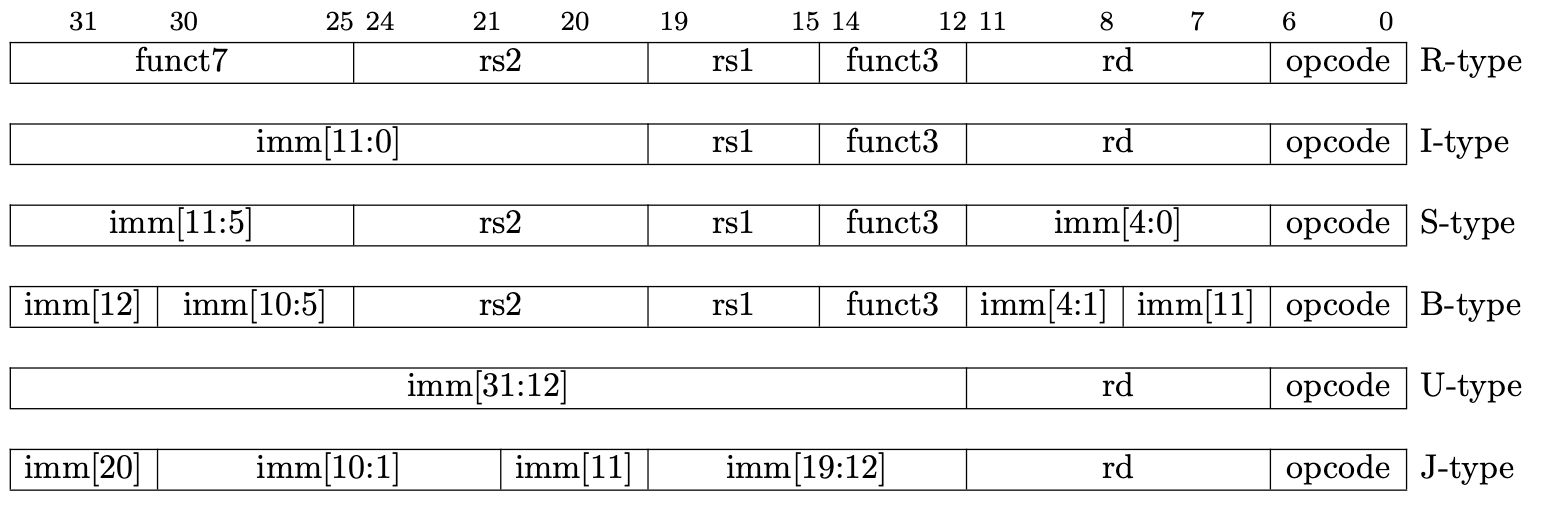
\includegraphics[draft=false,width=\linewidth]{chapters/chapter4/img/rv32i_instr_format.png}
    \caption{RV32I Base Instruction Formats}
    \label{table:rv32i_instr_format}
\end{center}
\end{table}

\subsection{Defining a RISC-V Custom Extension}
    \todo{I might need to make this its own section? At any rate, I need more background on what an instruction looks like etc}

    The goal of defining a custom extension in this context is to reduce the number of instructions neccesary to compute collisions for a given edge. According to RISC-V convention, the extension is designated \textbf{``Xedgcol''} (X for non standard, edgcol as an abbreviation for its purpose). When it is implemented along with RV32I, the processor can be said to implement the rv32i\_Xedgcol ISA.

    \subsubsection{Fixing Epsilon}
    Recall that the HoneyBee unit was parameterized for different values of $\epsilon$, and that this would influence the number of bits in its output sequence. When defining an instruction, this value has to be constant. You may have also noticed that the results presented for HoneyBee in Chapter 3 were all for $\epsilon = 4$. This value was chosen as $4^3 = 64$. Table \ref{table:epsilon_bits} lists the number of output bits required for each value of $\epsilon$ and how many 32-bit registers would be needed to store this result. From this, it is fairly obvious why 4 was chosen for the value of $\epsilon$.

    % @Author: AnthonyKenny98
% @Date:   2020-04-09 19:26:20
% @Last Modified by:   AnthonyKenny98
% @Last Modified time: 2020-04-09 20:07:12
\begin{table}[H]
\begin{center}
\begin{tabular}{|c|c|c|}
\hline
\textbf{$\epsilon$} & \textbf{Bits} & \textbf{Registers} \\
\hline
1 & 1 & 1/32 bits\\
\hline
2 & 8 & 8/32 bits \\
\hline
4 & 64 & 2 \\
\hline
6 & 216 & 6.75 \\
\hline
8 & 512 & 16 \\
\hline
\end{tabular}
\mycaption{Required Bits to Represent Output Collisions For Different Values of Epsilon}{. $\epsilon$ values of 1 and 2 underutilise both the register space available and the benefits of more parallelization that would come from larger values. Values larger than 4 would use up far too many of the available registers. $\epsilon = 4$ completely utilizes only two registers.}
\label{table:epsilon_bits}
\end{center}
\end{table}


    \subsubsection{Edge Collision Instruction}
    The following instruction was defined:

    \begin{center}
    \texttt{ecol rd1, rd2}
    \end{center}

    It takes two destination registers and stores result of the edge collision computation in them. The 32 \gls{LSB} are stored in \texttt{rd1} and the 32 \gls{MSB} in \texttt{rd2}.
    The instruction is formatted in the following way (For more detail, the full Xedgcol specification can be found in Appendix \ref{appendix:xedgcol_appendix}).

    \begin{table}[H]
    \begin{center}
    \begin{tabular}{c}
        \begin{tabular}{|m{0.2\linewidth}|m{0.1\linewidth}|m{0.1\linewidth}|m{0.1\linewidth}|m{0.1\linewidth}|m{0.1\linewidth}|}
        \hline
        \hspace*{0.5cm}000000000000 & \hspace*{0.5cm}rd2  & \hspace*{0.5cm}000  & \hspace*{0.5cm}rd1  & \hspace*{0.5cm}0000  & \hspace*{0.5cm}001  \\
        \hline
        \end{tabular} \\
        \begin{tabular}{m{0.2\linewidth}m{0.1\linewidth}m{0.1\linewidth}m{0.1\linewidth}m{0.1\linewidth}m{0.1\linewidth}}
        \hspace*{1.5cm}12 & \hspace*{0.5cm}5  & \hspace*{0.5cm}3  & \hspace*{0.5cm}5  & \hspace*{0.5cm}4  & \hspace*{0.5cm}3  \\
        \hspace*{1.3cm}null &  \hspace*{0.5cm}\textit{dest2} & \hspace*{0.5cm}null  & \hspace*{0.5cm}\textit{dest1}  &  \hspace*{0.5cm}null & \hspace*{0.25cm}ECOL  \\
        \end{tabular}
    \end{tabular}
    \end{center}
    \end{table}

    Conspicuously, the instruction specifies two destination registers, but no source registers. In other words, how does the processor know the coordinates of the edge? Also conspicuous is the fact that much of the instruction is null (meaningless zeros). Why not use this space to specify the coordinates of the edge?

    Consider, an edge must be represented by 6 32-bit numbers. This information, 192 bits in total, can not all fit in a single 32-bit instruction as 6 immediate values (obviously). Could those 32-bit values be stored in existing registers and the address of these registers referenced in the instruction? Since there are 32 general purpose registers in RISC-V, their addresses are 5-bits long each. 6 5-bit addresses is 30 bits in total, which, by itself could fit in an instruction. While this couldn't be combined with the edge collision instruction, perhaps a second instruction could be defined that contained the addresses of all 6, or even 3, of the registers containing the edge's coordinates. This was decided against for a few reasons, but mainly because \textbf{storing floating-point numbers in integer registers}, while theoretically possible, is extremely bad practice. To store floating point values in registers, a new register set would need to be defined.

    \subsubsection{Edge Registers}
